\section{Einführung}
\label{Einführung}
\subsection{Relevanz \& Problemstellung}
Bessere Code-Qualität mit im Vergleich minimal erhöhtem Zeitaufwand ist ein
erstrebenswertes Ergebnis, welches durch Test-driven Development (TDD) versucht
wird, zu erreichen. Durch die Idee von TDD - nämlich kurze Iterationen von:
\begin{enumerate}
  \item Tests schreiben (ohne sich Gedanken über den tatsächlichen Code zu machen)
  \item Tests ausführen und fehlschlagen lassen
  \item Code implementieren
  \item Tests ausführen und den Code eventuell weiter implementieren, bis die 
  Tests nicht mehr fehlschlagen
  \item Tests und Code refaktorieren
  \item Tests erneut ausführen
\end{enumerate}
wird eine hohe Testabdeckung und ein sauberer Code durch das Refaktorieren 
erzielt.

AngularJS ist ein umfassendes MVC Framework und bringt viele eigene Komponenten
mit sich, wie beispielsweise Direktiven und Services. Um test-driven mit 
AngularJS entwickeln zu können, ist es wegen der Vielfalt der eigenen 
Komponenten relevant, alle diese Komponenten testen zu können.

Mit der Relevanz von TDD mit AngularJS geht die Problemstellung der Auswahl 
eines passenden Testing Frameworks einher. Jasmine und Mocha sind zwei 
JavaScript Testing Frameworks, welche sich für diese Aufgabenstellung anbieten. 
Deshalb werden beide Frameworks in dieser Arbeit gegenüber gestellt und 
analysiert, um die Unterschiede beziehungsweise die Vor- sowie Nachteile jedes der 
Frameworks darstellen zu können.

\subsection{Methoden}
\subsubsection{Test-driven Development}
Eine theoretische Erfassung von Test-driven Development (TDD) und was die
Vor- und Nachteile von TDD verglichen mit anderen Entwicklungsmethoden sind, 
ist grundlegend für den weiteren Inhalt der Arbeit. Andere Entwicklungsmethoden
beinhaltet hier das Entwickeln ohne Testen sowie das Entwickeln und Testen im
nachhinein.

\subsubsection{AngularJS}
AngularJS wird zusammen mit den dazugehörigen Komponenten theoretisch und
praktisch dargestellt. Weitere Erläuterungen zu dem {\glqq 
Model-View-Controller (MVC)\grqq} Design-Pattern werden zum Verständnis des
Frameworks auch behandelt.
Die Theorie und die Praxis arbeiten hier sehr dicht zusammen, um im Vorfeld
alle Facetten des MVC-Frameworks abzuklären.

\subsubsection{Testing Frameworks}
Um abklären zu können, welches der beiden JavaScript Testing-Frameworks 
{\glqq Jasmine\grqq} und {\glqq Mocha\grqq} besser geeignet ist, um alle
Eigenschaften von AngularJS abzudecken, wird ein direkter theoretischer
Vergleich der Frameworks und deren Eigenschaften erfolgen. Darüber hinaus wird 
eine Applikation test-driven mit beiden Frameworks entwickelt. Die Applikation
wird alle der relevanten Eigenschaften von AngularJS behandeln. Der 
Entwicklungsprozess wird innerhalb der Arbeit dokumentiert.

\subsection{Forschungsfrage}
Wie ist der aktuelle Stand um AngularJS test-driven zu entwickeln und welches 
der beiden JavaScript Testing-Frameworks {\glqq Jasmine\grqq} und {\glqq 
Mocha\grqq} ist geeigneter für diesen Zweck?

\subsection{Begrifflichkeit}
 - Begrifflichkeit -

\newpage

\section{Test-Driven Development}
\label{section:Test-Driven Development}
\begin{center}
\glqq{\textit{Turning development upside-down}\grqq}\autocite[22]{Johansen:2011}
\end{center}
Traditionelle Entwicklungsmethoden stützen sich auf ein zuvor festgelegtes Konzept und eine passende Software-Architektur. Es wird so lange programmiert bis das Konzept durch Code und Architektur komplett abgebildet wird.

Test-Driven Development (TDD) dreht diesen Entwicklungsprozess um. Es fokusiert sich auf die Frage \glqq{Welchen Code benötige ich, um das Problem zu lösen\grqq}. TDD fokusiert sich hingegen darauf, als erstes das Ziel zu definieren. Danach gilt es, das Ziel mit so simplen Code wie möglich zu erreichen. Durch diesen Ansatz wird sichergestellt, dass nicht mehr Code als benötigt geschrieben wird. Das primäre Ziel von TDD ist nicht Testen, es gibt also auch bei TDD keine Garantie, dass Grenzfälle besser getestet werden. Dadurch, dass TDD zur simpelst möglichen Lösung führen soll, werden exzessive Code-Ausschweifungen unterbunden und dadurch wird Software robuster.

\subsection{Die zwei Regeln von TDD}
Für das Arbeiten mit TDD gelten zwei simple Regeln \autocite[]{Beck:2003}.
\begin{enumerate}
  \item Es wird nur neuer Code geschrieben, wenn einer der automatisierten Tests fehlschlägt.
  \item Dupplikationen werden eliminiert.
\end{enumerate}
Durch die Anwendung dieser einfachen Regel ergeben sich folgende Implikationen.
\begin{itemize}
  \item Es entsteht funktionierender Code, welcher in Kombination mit den Tests sofortiges Feedback zwischen Programmierentscheidungen liefert.
  \item Die Tests müssen von der/m EntwicklerIn selbst geschrieben werden. Die/Der EntwicklerIn kann selbstverständlich nicht auf Tester warten, denn sie/er ist abhängig von sfortigem Feedback um Programmierentscheidungen zu treffen.
  \item Die Entwicklungsumgebung muss auf jede Änderung schnell reagieren und das Feedback der Tests darstellen können.
  \item Um das Testen einfach zu halten muss hoch kohäsiver Code mit leicht gekoppelten Komponenten geschrieben werden.
\end{itemize}
Durch die Regeln sowie die Implikationen ergeben sich drei Aufgaben in folgender Reihenfolge.
\begin{enumerate}
  \item \textbf{Rot}: Einen kleinen Test schreiben.\newline
  Der kleine Test muss nicht erfolgreich durchgehen, ermuss auch noch nicht kompilieren.
  \item \textbf{Grün}: Den Test \textit{schnell} zum Laufen bringen.\newline
  Hier werden die einfachsten Änderungen welche sinnvoll erscheinen am Code vorgenommen um den zuvor erstellten Test erfolgreich abschließen zu können.
  \item \textbf{Refactor}: Alle Dupplikationen, welche durch das schnelle Hinzufügen von Code entstanden sind, eliminieren.
\end{enumerate}
Wenn es möglich ist, dieses theoretische Modell als Programmierungsstil umzusetzen, erhält man Code, welcher beinahe ausschließlich durch fehlgeschlagene Tests gefordert wurde. Die Anwendung dieses Programmierstils ergibt nicht nur die oben angeführten technischen, sondern ebenfalls soziale Implikationen.
\begin{itemize}
  \item Wenn die \textit{Fehlerdichte} möglichst gering gehalten werden kann, kann aus \textit{Qualitätssicherung} statt passiver zur aktiven Arbeit werden.
  \item Wenn die Anzahl von \textit{negativen Überaschungen} reduziert werden kann, wird der gesamte Entwicklungsprozess besser plan- und schätzbar.
  \item Da durch TDD sauberer Code entsteht, welcher zusätzlich durch Tests dokumentiert ist, kann die Kommunikation zwischen Software-EntwicklerInnen geschärft und klarer werden.
\end{itemize}

\subsection{Motivation: Angst {\&} Mut}
\cite{Beck:2003} stellt folgende Behauptung auf: \newline
\textit{TDD ist ein Weg um die Angst einer/s EntwicklerIn zurecht zu kommen}.

Hierbei geht es Beck um die legitime Angst einer/s EntwicklerIn \glqq{this-is-a-hard-problem-and-I-can't-see-the-end-from-the-beginning\grqq}. Durch diesen Ausdruck wird die Angst von einer zu großen und schwierigen Aufgabe erdrückt zu werden beschrieben.
Wenn ein/e EntwicklerIn sich mit diesem Problem konfrontiert sieht ergeben sich aus der Angst folgende negative Reaktionen.
\begin{itemize}
  \item Angst macht EntwicklerInnen \textit{zögerlich}.
  \item Angst macht EntwicklerInnen \textit{weniger kommunikativ}.
  \item Angst macht EntwicklerInnen \textit{scheu} vor \textit{Feedback}.
  \item Angst macht EntwicklerInnen \textit{mürrisch}.
\end{itemize}
Diese Reaktionen wirken sich alle negative auf die Code-Qualität sowie auf die Lösung des Problems aus.

Die richtigen Reaktionen wären jedoch folgende.
\begin{itemize}
  \item EntwicklerInnen sollten nicht zögern, sondern schnell und konkret an einem gegebenem Problem \textit{lernen und wachsen}.
  \item EntwicklerInnen sollten nicht schweigen und sich zurückziehen, sondern \textit{klarer kommunizieren}.
  \item EntwicklerInnen sollten aktiv nach \textit{konstruktivem Feedback} suchen.
\end{itemize}

Laut \cite{Beck:2003} werden diese Reaktionen durch TDD erreicht. Das große, erdrückende und angst-fördernde Problem wird zuerst durch viele kleine Tests ausgedrückt. Jeder Test wird der Reihe nacht zum Laufen gebracht. Wenn einer der Tests läuft, weiß die/der EntwicklerIn auch, dass der Test sowie der zugehörige Code funktioniert. Sie/er bekommt positives Feedback und kann sich auf das nächste Problem konzentrieren, wird also nicht mehr abgelenkt. Sollte dieser Test durch weitere Änderungen am Code fehlschlagen bekommt die/der EntwicklerIn direktes Feedback. Durch kleine Iterationen und simple Schritte können Fehler einfach gefunden werden.

Weiters beschreibt Beck TDD als Bewusstsein der Lücke zwischen Programmierentscheidungen und Feedback sowie die Möglichkeiten um diese Lücke kontrollieren zu können.

\subsection{Der TDD-Kreislauf}
\begin{enumerate}
  \item \textbf{Test schreiben}:\newline
  Der Test sollte wiederspiegeln, wie ein/e EntwicklerIn sich die zukünftige Operation wünscht. Der Test ist eine Geschichte. Diese Geschichte soll alle möglichen Elemente beinhalten, welche notwendig sind um die richtigen Antworten für die Geschichte zu erhalten.
  \item \textbf{Test zum Laufen bringen}:\newline
  Den Test \textit{schnell} zum Laufen bringen ist das Wichtigste. Wenn eine klare, saubere Lösung offensichtlich ist, dann spricht nichts dagegen diese auch zu implementieren. Wenn diese Lösung jedoch zu lange dauert, um den Test \textit{schnell} zum Laufen zu bringen - also das \glqq{grüne\grqq} Feedback verzögern - sollte eine Notitz erstellt werden und die Konzentration sofort wieder auf das eigentliche Problem gelenkt werden. Oft werden hier auch \glqq{Fake\grqq} Implementierungen angewendet.
  \item \textbf{Es richtig machen}:\newline
  Schritt für Schritt können nun Duplikationen entfernt sowie etwaige \glqq{Fake\grqq} Implementierungen aus Schritt 2 behoben werden.
\end{enumerate}

Das Ziel dieser drei Schritte ist \glqq{clean code that works\grqq}, also \glqq{\textit{sauberen}, \textit{funktionierenden} Code\grqq} zu erhalten.

Folgendes Beispiel illustriert diesen Kreislauf anhand einer einfachen Implementierung für simple Addition.
Die erläuternde Beispiele zu TDD werden in JavaScript verfasst, da sich diese Arbeit primär mit JavaScript und AngularJS befasst.
Das Beispiel kann im referenziertem GitHub-Repository in dem Verzeichnis \glqq{source/simple-tests/step-1\grqq} gefunden werden.

Schritt 1: Test schreiben.
Der erste einfache Test beschreibt eine Geschichte. In dieser Geschichte soll die Funktion \glqq{plus(arg1, arg2)\grqq} die zwei übergebenen Parameter addieren und ein Ergebnis zurückliefern. Für die einfachste Integer-Variante bedeutet das also: \glqq{1+1=2\grqq}

\begin{lstlisting}[style=verbo]
describe("Calculus - Simple addition", function() {

  it("should add 1 to 1 and return 2", function() {
    expect(plus(1,1)).toEqual(2);
  });

});
\end{lstlisting}

Dieser Test wird per Kommandozeile im Browser \glqq{PhantomJS\grqq} ausgeführt. Der Befehl dafür lautet: \glqq{karma start karma-simple.conf.js\grqq}. Der erste Test ist geschrieben, jedoch gibt es noch keine Implementierung, dass heißt hier wird ein negatives Testergebnis erwartet. Das erwartet Ergebnis ist auf Abbildung \ref{figure:tdd-simple-step-1-1} zu sehen.

\begin{figure}[H]
  \centering
  \fbox{
  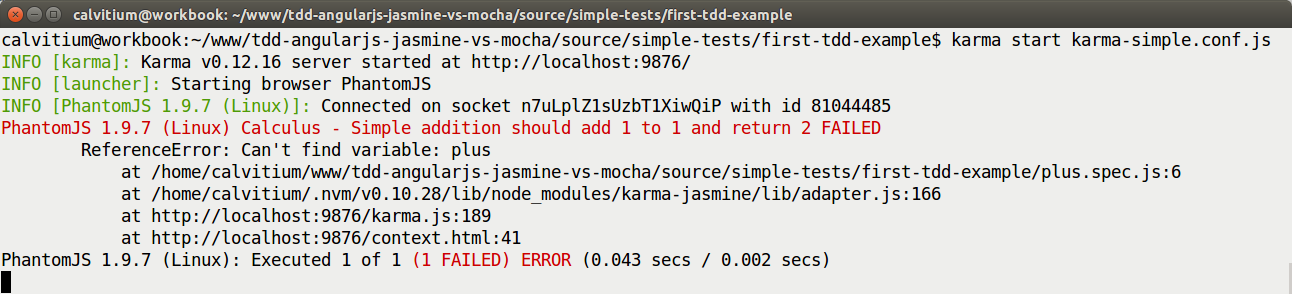
\includegraphics[width=12cm]{images/tdd-simple-step-1-1.png}
  }
  \caption{Terminal Ausgabe des ersten Tests}
  \label{figure:tdd-simple-step-1-1}
\end{figure}

Schritt 2: Zum Laufen bringen.
Um diesen Test möglichst schnell dazu zu bringen grünes Feedback zu geben, wird die einfachste und naiivste Implementierung verwendet.
Die einfachste Variante bedeutet also eine Funktion zu definieren, welche zwei Parameter übernimmt und \glqq{2\grqq} zurückgibt.

\begin{lstlisting}[style=verbo]
var plus = function(augend, addend) {
  return 2;
};
\end{lstlisting}

Wir wissen an dieser Stelle natürlich, dass hier eine klare, saubere und offensichtliche Lösung existiert. Es spricht natürlich nichts dagegen diese hier auch anzuwenden, um jedoch auch den dritten Schritt illustrieren zu können, wird hier naiv vorgegangen.\newline
Nach dieser naiven Implementierung ändert sich das Ergebnis des Tests von rot auf grün (siehe Abbildung \ref{figure:tdd-simple-step-1-2}).

\begin{figure}[H]
  \centering
  \fbox{
  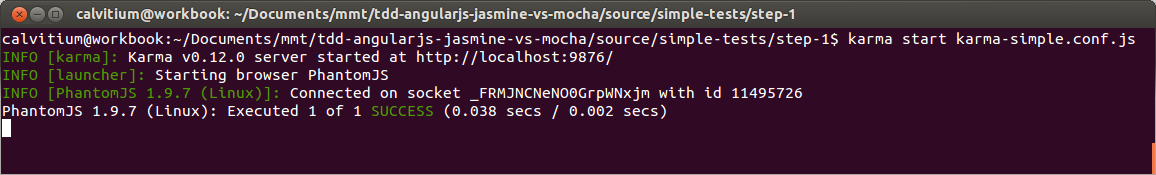
\includegraphics[width=12cm]{images/tdd-simple-step-1-2.png}
  }
  \caption{Terminal Ausgabe des ersten Tests nach naiver Implementierung}
  \label{figure:tdd-simple-step-1-2}
\end{figure}

Schritt 3: Es richtig machen.
Obwohl der Test nun bereits erfolgreich läuft, ist natürlich klar, dass diese naive Implementierung nicht korrekt ist. Es handelt sich um eine \glqq{Fake\grqq} Implementierung. Um nun die richtige Berechnung durchzuführen ändern wir die \glqq{plus(arg1, arg2)\grqq} Funktion folgendermaßen.

\begin{lstlisting}[style=verbo]
var plus = function(augend, addend) {
  return augend+addend;
};
\end{lstlisting}

Nach dem dritten Schritt wird erneut der Test ausgeführt um zu garantieren, dass das Korrigieren der naiven Implementierung auch funktioniert. Es wird ein positives Ergebnis erwartet (siehe Abbildung \ref{figure:tdd-simple-step-1-3}).

\begin{figure}[H]
  \centering
  \fbox{
  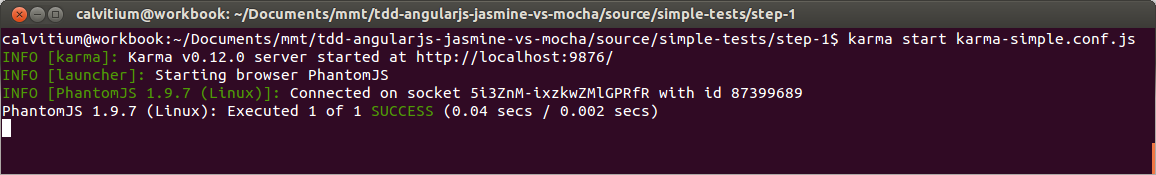
\includegraphics[width=12cm]{images/tdd-simple-step-1-3.png}
  }
  \caption{Terminal Ausgabe des ersten Tests nach Richtigstellung der Implementierung}
  \label{figure:tdd-simple-step-1-3}
\end{figure}

Durch die Anwendung des TDD-Kreislaufs wurde hier \textit{sauberer} und \textit{funktionierender} Code produziert.\newline\newline

\subsection{Test-Driven Development Patterns}
\subsubsection{Red Bar Patterns}

Diese Muster betreffen den ersten Teil des TDD-Kreislaufs: das Test Schreiben.
Konkret behandeln sie die Fragen:
\begin{itemize}
  \item \glqq{Wann\grqq} sollen Tests geschrieben werden?
  \item \glqq{Wo\grqq} sollen Tests geschrieben werden?
  \item \glqq{Wann\grqq} soll mit dem Tests Schreiben \glqq{aufgehört\grqq} werden?
\end{itemize}

\textit{One Step Test}

Bei TDD handelt es sich wie bereits erwähnt um einen Prozess, bei welchem in kleinen Schritten und Schritt für Schritt Software aus Tests geformt wird. In diesem Prozess ist es notwendig sich für die Reihenfolge der Test-Schritte (in weiterer Folge auch für die Reihenfolge, in welcher die Komponenten der Software entstehen soll) zu entscheiden.

\cite[134]{Beck:2003} liefert auf die Frage \glqq{Welchen Test sollte ich als nächstes schreiben?\grqq} eine klare Antwort: Es gibt keine.
Die Frage ist hinsichtlich der Anforderungen der Software (beziehungsweise deren Komponenten) sowie der/s Entwicklerin/s zu individuell.
Beck gibt jedoch den Tipp, weder Tests mit einer offensichtlichen Implementierung, noch Tests, welche zu kompliziert erscheinen zu wählen.
Man sollte Schritt für Schritt jene Tests wählen, bei welchen man sich wohlsten fühlt.
Sollten nur zu komplizierte Probleme und Tests vorliegen müssen die Schritte verkleinert und somit das Szenario noch weiter unterteilt werden.

Die Mechanik des \glqq{One Step Test\grqq}'s wird von \cite[134]{Beck:2003} mit \glqq{known to unknown\grqq} beschrieben.\newline\newline

\textit{Starter Test}

Mit welchem Test soll begonnen werden?

Eines der Grundkonzepte von TDD besagt, dass die Konzentration immer nur auf dem aktuellen Problem und Test liegen soll. Diesem Konzept steht jedoch die Möglichkeit mit einem realistischen Test zu starten gegenüber. Bei dem Versuch einen realistischen Test zu schreiben, wird der Fokus sofort auf einige andere Fragen gelenkt. \glqq{Was ist der richtige Input?\grqq}, \glqq{Was ist das richtige Ergebnis?\grqq}, \glqq{Welche Parameter sind notwendig für Lösung des Problems?\grqq} oder \glqq{Wohin gehört dieser Test eigentlich?\grqq}. Man findet sich bei dem Schreiben realistischer Tests häufig dabei wieder über viele Probleme und Fragen auf einmal nachzudenken, verliert also den Fokus auf den aktuellen Test des aktuellen Problems.

Ein realistischer Test bedeutet eine Verzögerung des Abstands der \glqq{Rot-Grün-Refactor\grqq} Zyklen - diese sollen jedoch möglichst kurz gehalten werden.
Der erste Test, also der \glqq{Starter Test\grqq} soll so trivial wie möglich sein.

\glqq{Start by testing a variant of an operation that doesn't do anything\grqq}, \cite[134]{Beck:2003}.\newline\newline

\textit{Learning Test}

Wie bereits erwähnt geht es bei TDD nicht nur um eine möglichst hohe Test-Dichte, sondern ebenfalls um andere Faktoren, wie Design, Schätzbarkeit, sauberen Code, psychologische Auswirkungen, etc.

Eine weitere Methode TDD einzusetzen betrifft das Lernen des Umgangs mit einer neuen API oder Bibliothek. Wenn man eine neue Bibliothek verwendet bietet es sich an, gegen diese Tests zu schreiben anstatt direkt Implementierungen damit vorzunehmen - ansonsten sollten keine Tests für externe Software mptwendig sein.\newline\newline

\textit{Regression Test}
Wenn ein Fehler in einer Applikation auftritt, so ist eine Variante dieses Problem zu lösen direkt den Fehler zu finden, zu behen, zu überprüfen und damit den Fehler abzuhaken. Mit dieser Variante gib es allerdings keine Möglichkeit zu garantieren, dass dieser Fehler (durch Abhängigkeiten zu anderen Komponenten) nicht erneut auftritt.

Auch TDD kann keine 100\%-ige Fehler-Freiheit garantieren. Sollte ein Problem berichtet werden, ist der erste Schritt einen neuen Test für dieses Problem zu verfassen. Der Test muss den einfachsten Fall, welcher das Fehlverhalten hervorruft behandeln. Durch das nachträgliche absolvieren des TDD-Kreislaufs wird sichergestellt, dass genau dieser Fehler nicht erneut auftritt.

\subsubsection{Green Bar Patterns}

Die \glqq{Red Bar Patterns\grqq} helfen dabei die notwendigen Tests zu verfassen. Die \glqq{Green Bar Patterns\grqq} hingegen geben nun Ansätze, wie die geschriebenen und fehlschlagenden Tests schnellst möglich erfolgreich abgeschlossen werden können.\newline\newline

\textit{Fake it ('til you make it)}

Um die Abstände der \glqq{Rot-Grün-Refactor\grqq} Zyklen so gering wie möglich halten zu können wird immer die einfachste Variante aller möglichen Implementierungen verwendet: Eine Konstante zurück liefern.

Nachdem der Test grün ist wird Schritt für Schritt die Implementierung richtig gestellt und die Konstante mit Variablen in einen Ausdruck gewandelt. Hier stellt sich jedoch die Frage \glqq{Wieso offensichtlich falschen Code schreiben?\grqq} - Um den Test schnell erfolgreich laufen lassen zu können.
Laut \cite[152]{Beck:2003} hat dieses Muster zwei starke Effekte. Wenn der Test grün ist fühlt man sich sicher. Man kann sich voll und ganz auf das richtige Refaktorieren konzentrieren. Also einerseits erfüllt \glqq{Fake it\grqq} einen psychologischen Effekt. Andererseits hilft es bei der Abgrenzung von zukünftigen Problemen. Wie schon erwähnt dient TDD auch dazu den Fokus und die Konzentration immer bei dem aktuellen Problem zu halten. Als ersten Schritt eine Konstante zurück zu liefern unterstützt dabei die/den EntwicklerIn.

BAIIISPÜÜÜÜL + Duplikation zwischen Test \& Implementierung removen undso.\newline\newline

\textit{Triangulate}

Ein weiterer Weg um schnell einen erfolgreichen Test zu erreichen ist \glqq{Triangulate\grqq}. Bei Triangulate geht es darum, nicht nur ein mögliches Ergebnis zu testen, sondern zwei oder mehrere Ergebnisse.

Anhand des folgenden Beispielswird der direkte Unterschied zu \glqq{Fake it\grqq} erklärt.

BAIIISPÜÜÜÜÜHL

Bei Triangulate wird also nicht mittels direkter Eliminierung der Duplikation zwischen Test und Implementierung refaktoriert, sondern durch das Hinzufügen eines weiteren möglichen Ergebnisses.\newline\newline
\newpage
\textit{Obvious Implementation}

Wie die bisherigen Beispiele für \glqq{Fake it\grqq} und \glqq{Triangulate\grqq} zeigen, handelt es sich dabei um wirklich kleine Schritte. Speziell anhand dieses Beispiels lässt sich das dritte Green Bar Patterns erklären: \glqq{Obvious Implementation\grqq}.

Wenn eine Operation so einfach ist, wie in dem Beispiel, spricht nichts dagegen die offensichtliche Implementierung direkt zu verwenden.
Wenn die Probleme allerdings komplizierter werden, ist es oft schwierig die Disziplinen \glqq{sauberer\grqq} und \glqq{funktionierend\grqq} gleichzeitig zu erreichen. Außerdem soll der Abstand zwischen den Zyklen möglichst gering gehalten werden, was bei einer offensichtlichen Lösung für ein großes Problem eventuell nicht eingehalten werden kann.

BAISPÜÜÜÜHL\newline\newline

\textit{One to many}

Auch bei Operationen, welche eine Kollektion von Objekten benötigen, gilt: einfach und simpel starten - \glqq{one to many\grqq}\autocite[154]{Beck:2003}.

Zuerst erfolgt die Implementierung mit einem Objekt und erst wenn der Test erfolgreich war wird Schritt für Schritt die Kollektion übernommen.

BEISPÜÜÜÜÜHL - Beachten: Änderungen Isolieren
\newpage

% 2168 - 2239 Wöter (36 Code)

\subsection{Testing}
 - kurze Testing Einleitung - (verschiedene Varianten, verschommene Varianten durch ähnliche Bezeichnungen, (integration/e2e, etc.))

\subsubsection{Unit-Tests}
Ein Unit-Test ist Code, welcher produktiven Code testet. Er besteht aus bestimmten Objekten in bekannten Stati. Die Objekte, wie beispielsweise Funktionen, werden ausgeführt. Dnach werden sie inspiziert und/oder auf die Richtigkeit überprüft. Der produktive Code wird in Isolation getestet.

Im Vergleich zu Integration-Tests ist es für Unit-Tests wichtig, dass sie isoliert ausgeführt werden - kein Test soll von einem anderen Test abhängig sein \autocite[4]{Johansen:2011}. Langsame Unit-Tests sind schlecht. EntwicklerInnen werden langsame Tests nicht so oft ausführen wie schnelle Tests. Insbesondere im Zusammenhang mit TDD bedeuten langsame Tests einen längeren Abstand zwischen den TDD Zyklen. EntwicklerInnen müssen lange auf Feedback warten und werden aus dem Zyklus gerissen.

Unit-Tests können zu jeder Zeit ausgeführt werden.
\begin{itemize}
  \item Um bei einer fertigen Implementierung deren Korrektheit bestätigen.
  \item Um bei Änderungen Fehler auszuschließen.
  \item Um bei dem Hinzufügen von neuen Komponenten zu garantieren, dass das System noch vollständig und richtig funktioniert.
\end{itemize}

 - Abgrenzung von Unit-Tests -

\subsubsection{Integration-Tests}
Um beispielsweise eine Uhr zu testen, benötigt man beides, Unit- sowie Integration Tests. Unit-Tests sind für das Testen der einzelnen Zahnräder der Uhr zuständig. Diese werden isoliert auf ihre Korrektheit getestet. Integration-Tests hingegen testen, wie die Zähne der einzelnen Zahnräder ineinandergreifen und ob die Uhr als ganzes richtig funktioniert.

Der Nachteil von Integrations-Tests ist, dass diese im Vergleich zu Unit-Tests eher langsam sind. In der Web-Entwicklung werden Integrations-Tests oft verwendet, um die korrekte Darstellung von Elementen sicherzustellen, oder um die Korrektheit der Routen der Web-Applikation zu testen. (Da fällt mir bestimmt auch noch was ein). Das Inspizieren der DOM verlangsam auch die Integrationstests.

\subsubsection{Automatisiertes Testen in der Web-Entwicklung}
Beim Entwickeln einer Web-Applikation gibt es ein Schema, welches jeder/m WebentwicklerIn bekannt ist. Man schreibt in einem Text-Editor oder in einer IDE Code, wechselt (ALT+TAB) auf den aktuellen Browser, erneuert die Seite (F5) und überprüft manuell den soeben geschriebenen Code. Dieses Schema ist sehr zeitintensiv, fehleranfällig und nicht reproduzierbar \autocite[3]{Johansen:2011}. Darüber hinaus reicht es oft nicht, den geschriebenen Code lediglich in einem Browser zu testen.

Durch TDD wird dieses Schema vereinfacht. Die meisten Test-Runner (<- Begrifflichkeit), wie beispielsweise \glqq{Karma\grqq}, bieten Funkionalität an, um Dateien auf Änderungen zu überwachen. Sobald eine Änderung stattgefunden hat werden sofort alle Tests erneut ausgeführt. Viele Test-Runner bieten außerdem die Möglichkeit, in mehreren verschiedenen Browsern automatische Tests laufen zu lassen. Die Auswahl reicht von den gängigen Browsern \glqq{Google's Chrome\grqq}, \glqq{Mozilla's Firefox\grqq}, \glqq{Apple's Safari\grqq} und \glqq{Microsoft's Internet Explorer\grqq} über den bei Web-EntwicklerInnen beliebten \glqq{Google's Chrome Canary\grqq} bis hin zu \glqq{headless\grqq} Browsern (-> Begrifflichkeit) wie beispielsweise \glqq{PhantomJS\grqq}.

Durch TDD und automatische Tests wird die Zeit für das manuelle Testen eingespart. Die Tests sind reproduzierbar und die Implementierungen sind weniger fehleranfällig. Das Ergebnis ist also ein effizienterer Entwicklungsprozess.

In Kombination mit gewissen Frameworks, zum Beispiel Karma, kann darüber hinaus direktes automatisches Feedback für die/den EntwicklerIn durch das Überwachen der Dateien erreicht werden. Das manuelle Testen in verschiedenen Browsern wird ebenfalls von Karma übernommen.

\subsection{Vorteile von TDD}
\label{Vorteile von TDD}
Die bisherigen Kapitel dieser Arbeit erläutern die Prozesse, Funktionsweisen, Auswirkungen sowie Pattern von TDD. Dieses Kapitel fasst die wichtigsten Vorteile von TDD zusammen.
\begin{itemize}
  \item \textbf{Funktionierender Code}\newline
  Durch die hohe Test-Dichte wird die Fehleranfälligkeit verringert und die Stabilität der geschriebenen Software erhöht. Der TDD Zyklus \glqq{zwingt\grqq} EntwicklerInnen förmlich dazu, anhand von Tests vor der Implementierung darüber nachzudenken.
  \item \textbf{Sauberer Code}\newline
  Sauberer Code durch refactoring. Durch TDD wird refactoring automatisch in den Entwicklungsprozess integriert (siehe Green Bar Patterns). Durch die zuvor entstandenen Tests wird in diesem Schritt garantiert, dass sich durch das refactoren keine Bugs einschleichen. Weiters wird durch TDD die Wertschätzung des \glqq{Single Responsibility\grqq} Prinzips und die lose Kopplung der Komponenten gefördert\autocite[30]{Johansen:2011}.
  \item \textbf{Psychologische Effekte}\newline
  Das positive Feedback wirkt sich positiv auf das Stresslevel von EntwicklerInnen aus.
  TDD hilft dabei sich nur auf das aktuelle Problem zu konzentrieren und sich von zukünftigen Problemen und Entscheidungen abzugrenzen.
  \item \textbf{Dokumentation}\newline
  Mit TDD wird Software aus Tests geformt. Tests wiederrum \glqq{erzählen\grqq} eine Geschichte. Sie spiegeln die Anforderungen und die vorgesehen Implementierung einer Komponente wieder. Tests können somit auch eine gewisse Dokumentationsfunktion erfüllen und zur besseren Verständnis von Software und einzelnen Komponenten beitragen.
  \item \textbf{Produktivität}\newline
  Das Hauptargument gegen TDD lautet: TDD benötigt Zeit und muss gelernt werden.
  Ist TDD jedoch einmal gelernt und wird regelmäßig angewandt sorgt es durch alle bisher genannten Vorteile für einen Produktionsschub.
\end{itemize}

% Words in text: 3149
% Words in headers: 82
% Words in float captions: 22


\subsection{Andere Entwicklungsmethoden}
 - Andere Entwicklungsmethoden - 
\subsection{Gegenüberstellung}
 - Gegenüberstellung -

\newpage
\section{AngularJS}
 - AngularJS -

\subsection{Hintergründe}
 - Hintergründe -
\subsection{Anatomie von AngularJS}
 - Anatomie von AngularJS -
\subsection{Model-View-Controller Design Pattern}
 - Model-View-Controller Design Pattern -
\subsection{Komponenten}
 - Komponenten -

\subsubsection{Controller}
 - Controller -
\subsubsection{Directives}
 - Directives -
\subsubsection{Services}
 - Services -
\subsubsection{Dependency-Injection}
 - Dependency-Injection -
\subsubsection{Data-Binding}
 - Data-Binding -

\subsection{Entwickeln mit AngularJS}
 - Entwickeln mit AngularJS -

\newpage
\section{Testing Frameworks}
 - Testing Frameworks -

\subsection{Jasmine}
 - Jasmine -

\subsubsection{Hintergründe}
 - Hintergründe -
\subsubsection{Funktionen}
 - Funktionen -
\subsubsection{Testen von asynchronem Javascript}
 - Testen von asynchronem Javascript -

\subsection{Mocha}
 - Mocha -

\subsubsection{Hintergründe}
 - Hintergründe -
\subsubsection{Funktionen}
 - Funktionen -
\subsubsection{Testen von asynchronem Javascript}
 - Testen von asynchronem Javascript -

\subsection{Gegenüberstellung}
 - Gegenüberstellung -
\newpage
\section{Conclusio}
 - Conclusio -

\newpage
\section{Ausblick}
 - Ausblick -

\nocite{Green:2013}
\nocite{Kozlowski:2013}
\nocite{Hahn:2013}
\nocite{Zakas:2012}
\nocite{MacCaw:2011}
\nocite{Burnham:2011}
\nocite{Gaertner:2012}
